\documentclass[11pt]{article}

\newcommand{\squishlist}{
   \begin{list}{$\bullet$}
    { \setlength{\itemsep}{0pt}      \setlength{\parsep}{3pt}
      \setlength{\topsep}{3pt}       \setlength{\partopsep}{0pt}
      \setlength{\leftmargin}{1.5em} \setlength{\labelwidth}{1em}
      \setlength{\labelsep}{0.5em} } }

\newcommand{\squishend}{
    \end{list}  }

\usepackage{times}
\usepackage{mathptm}
\usepackage{fullpage}
\usepackage{graphicx}\usepackage{url}

\begin{document}

\begin{center}
{\bf{Regis University -- Physics 305A -- Fall 2019}} \\
{\bf{Lab 3: Force Table}} \\
\medskip
\textbf{Part I: Forces on a Force Table}
\end{center}

\medskip

In this lab, you will begin to build your physical intuition about forces and 
improve your ability to calculate with vectors.

You probably have some intuition about forces from your everyday experience. For example, you probably have a rough idea that they are the interactions that cause objects tol accelerate -- if you push on a shopping cart (i.e., apply a force), the shopping cart starts accelerating. In lecture, you will soon start studying forces in more formal detail. For now, we will simply make note of the fact that forces are \textbf{vectors}: they have a magnitude and direction. When the sum of forces on an object (the ``net force'') is equal to zero, the object will not accelerate. We will explore this fact today as a means for practicing vector math. You will try to balance the forces (i.e., make them sum to zero) due to gravity acting on small masses by using a force table.

There is one important fact that you will likely need to being to set up this experiment: The gravitational force on a mass within Earth's gravitational influence near the planet's surface can be calculated as 
\begin{equation}
\vec{F}=m\vec{g},
\end{equation}
where $m$ is the object's mass and $|\vec{g}|=9.8~\rm m/s^2$ is the gravitational acceleration due to Earth. This simple relationship allows you to relate an object's mass to its weight (i.e., force) if it is near Earth's surface. In our experiment, this force acts on each small mass and is transmitted to a small metal ring via tension in a string.

\bigskip

\begin{center}
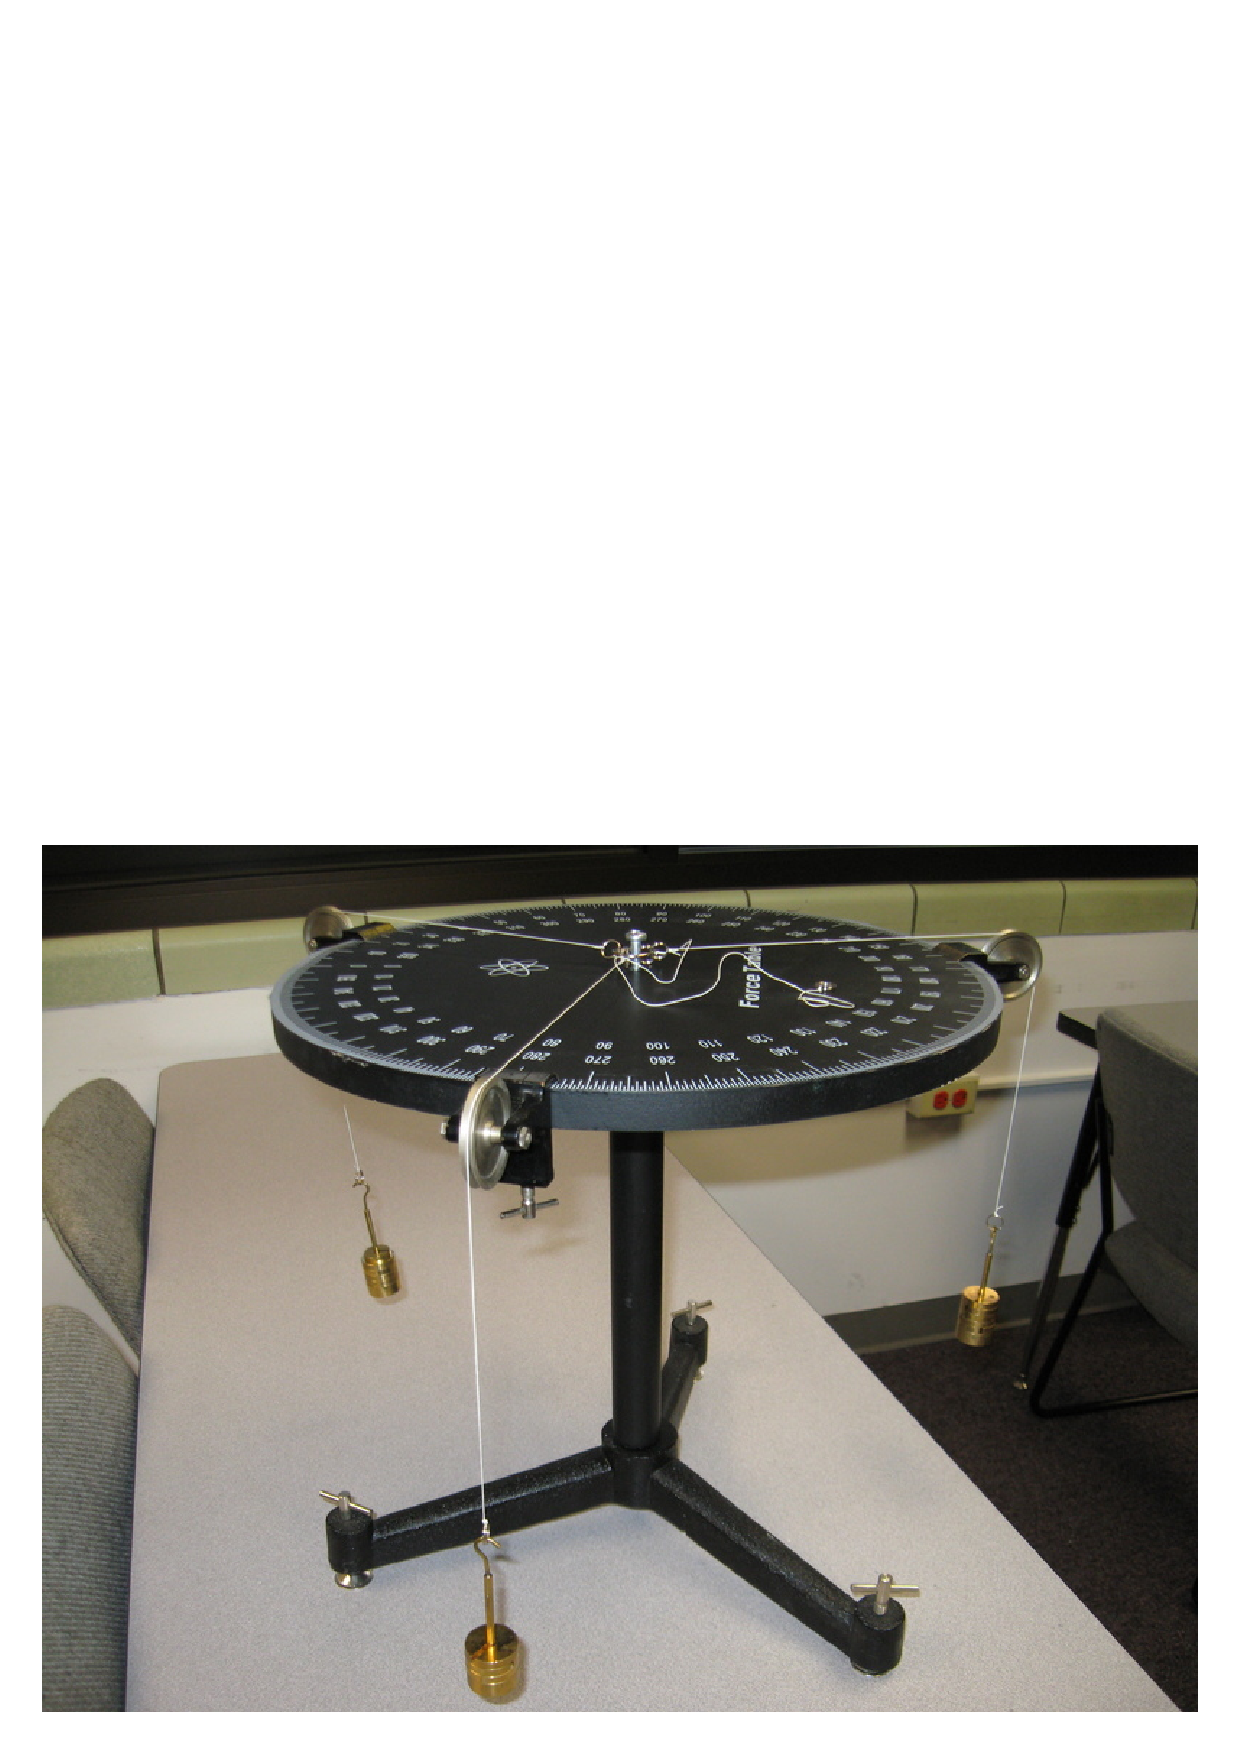
\includegraphics[height=0.30\textheight]{force_table_side1.pdf}
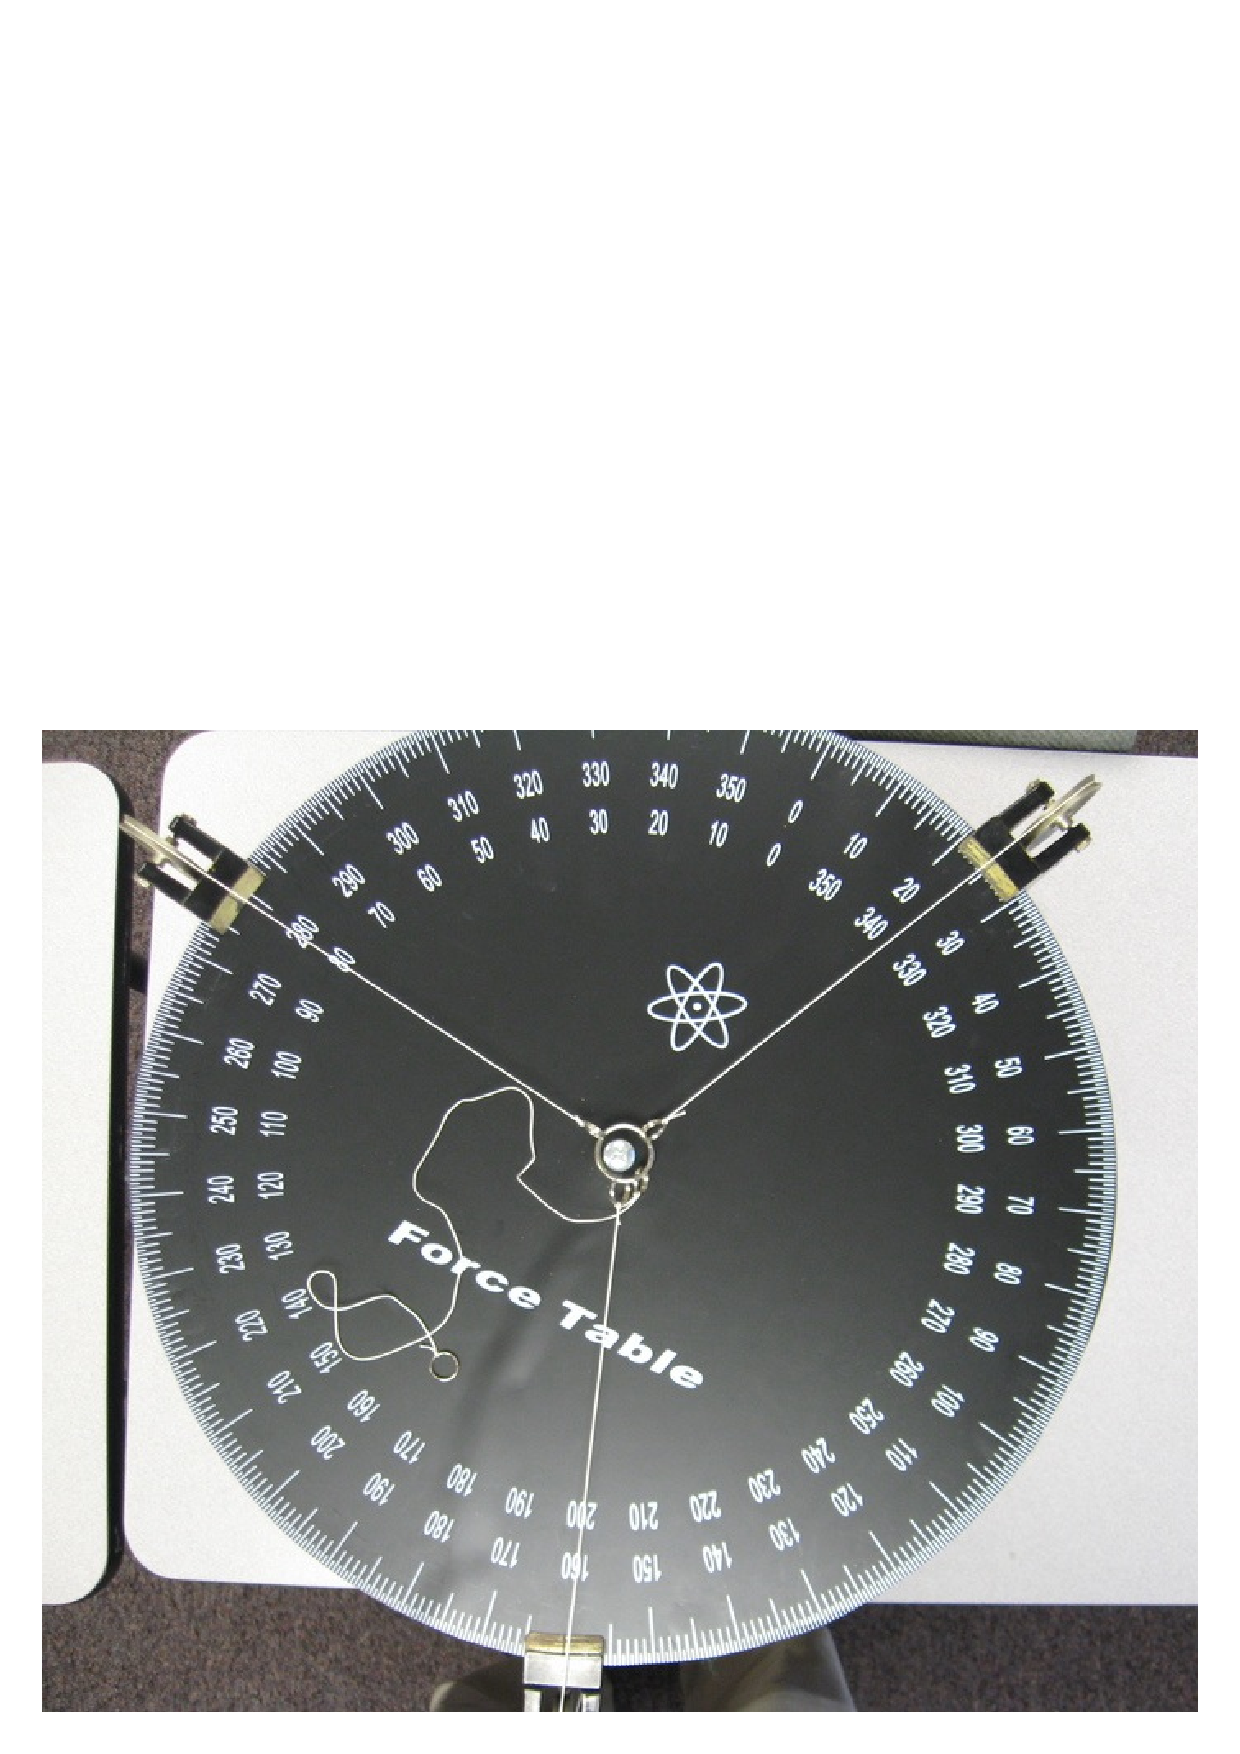
\includegraphics[height=0.30\textheight]{force_table_top1.pdf}
\end{center}

The force table is shown ``in action'' in the photographs above; we have a 
number of models that look somewhat different, but the basic principle is 
the same.  It is marked with an angular scale.  Pulleys can be clamped onto
it at any position around the circumference, allowing you to hang masses
on strings from any angle.  These strings are linked together by a ring;
your goal is to find a configuration in which the net force on the ring 
is zero (well, at least very small) so that it remains balanced, 
in static equilibrium.
\newpage

\small

The table below specifies the magnitude and direction of two forces for
various force table ``problems'':

\begin{center}
\begin{tabular}{l|ll|ll}
\hline
Problem & Force 1 & Angle 1 & Force 2 & Angle 2 \\
\hline
A & 1.22~N  & 0$^\circ$ & 1.47~N & 85$^\circ$ \\
B & 0.88~N & 75$^\circ$ & 1.76~N & 165$^\circ$ \\
C & 1.47~N & 30$^\circ$ & 1.47~N & 118$^\circ$ \\
D & 1.96~N & 0$^\circ$ & 2.16~N & 120$^\circ$ \\
\hline
\end{tabular}
\end{center}




\noindent For each of the problems:
\begin{enumerate}
\item Compute the magnitude and direction of a third force that would 
counterbalance the given pair, giving a net force
${\vec F}_{net} = {\vec F}_1 + {\vec F}_2 + {\vec F}_3 = \vec 0$.
Remember that, to add vectors, you must break them into their Cartesian
components and add those components.
\item Determine how much mass to hang at each position 
 to create each of these three forces: two that were given, and one that
 you just calculated.
\item Set up the force table as you have calculated.  Is the system balanced
  in static equilibrium, with the ring stationary at the center of the table?  
\item If not, you should first double-check your calculations.  If they are 
  correct, then you should be able to make it balance with a small 
  adjustment to one of the forces.  How large was this adjustment,
  as a percentage of the force itself?
\end{enumerate}  
\begin{center}
\textbf{Part II: Computational Activity 2}
\end{center}
Do not begin this part until you have completed all calculations in Part I. Handheld calculators are horribly inefficient for doing repetitious calculations, like you did in Part I. By writing a small computer program, you can do multiple complex calculations quickly. In this part, you will write a Python program to automate what you did manually in Part I.

\begin{center}
\begin{tabular}{l|ll|ll}
\hline
Problem & Force 1 & Angle 1 & Force 2 & Angle 2 \\
\hline
E & 1.47~N  & 0$^\circ$ & 1.22~N & 85$^\circ$ \\
\hline
\end{tabular}
\end{center}

Your job is to use the Python skills that you began to learn in Lab 1 to write a program that solves Problem E below in the same way that you solved the above problems manually. I've given you a skeleton of the code below; you must finish and adapt it. In doing so, you will definitely want to make use of the functions \texttt{math.pi}, \texttt{math.sin()}, \texttt{math.cos()}, and \texttt{math.atan()}, all of which you can google if you have questions about them. (Hint: Do these trig functions accept degrees or radians as input?) Also remember that lines that begin with \# are comments; Python \textbf{ignores} them entirely. You need to uncomment a line if you want Python to use it. My skeleton of code below is just a suggestion; feel free to modify and experiment. However, you should obtain working code before you turn in your lab report, and you lab report should contain all of the code you wrote. If you do not finish it in lab, you should finish it before next lab. 

As we discussed in Lab 1, you can run Python natively on your computer, but most of you probably don't have it installed, so we'll use a website that runs your code online for you. If you happen to have Python installed or prefer a different online implementation, feel free to use those. Regarless, please go to \url{https://trinket.io/python3/12950deb2c} to get my skeleton code.  

If you feel confused by this exercise, please don't worry. Everyone makes a mess of programming the first time they attempt it. Try to enjoy the experimentation, failure, and learning!

When you are finished, please take a moment to appreciate what you have done. Though it was hard to code, you have now solved \textbf{all possible} three-vector problems. If you did it right, you could change the input values to any others and \textbf{instantly} get the answer! 


\end{document}
